%----------------------------------------------------------------------------------------
%----------------------------------------------------------------------------------------
%----------------------------------------------------------------------------------------
%DATA
%----------------------------------------------------------------------------------------
%----------------------------------------------------------------------------------------
%----------------------------------------------------------------------------------------

\section{DATA}
\label{sec: data}
We use SED templates from \citealias{Kinney96} to train neural networks.
To test the trained networks, we use SED and physical properties of 142 galaxies at $0.5<z<1$ from \citealias{Hossein12}.
Following the \citealias{Hossein12} work, we chose these two sets of data not only to show the application of SOMs in SED clustering, but also to easily compare supervised and unsupervised methods.

 \subsection{Kinney spectral model}
     \begin{figure}
        \centering
        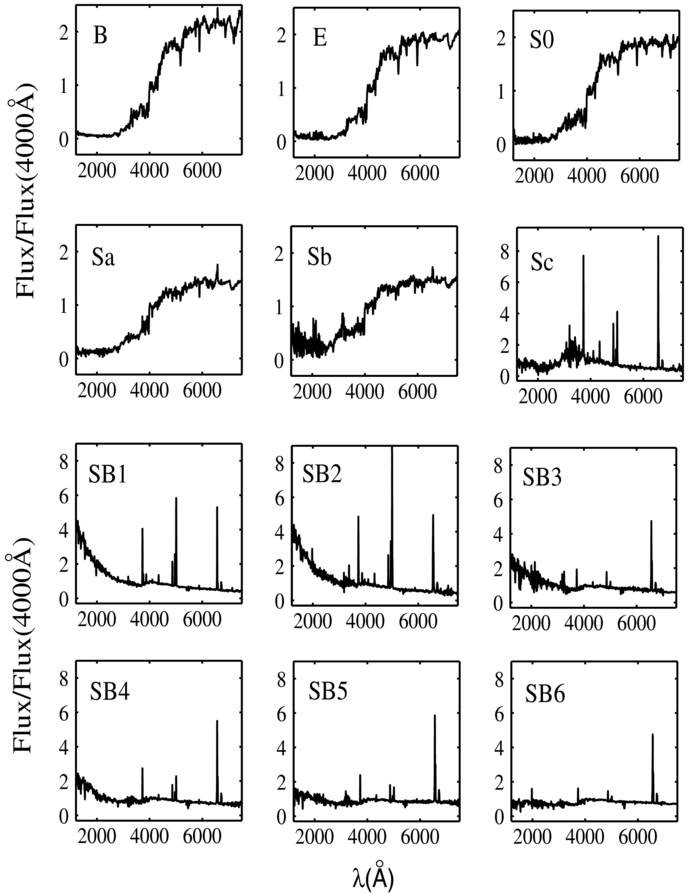
\includegraphics[width=0.5\textwidth]{images/k96.jpg}
        \caption{\citealias{Kinney96} spectra template for 12 types of galaxies from \citealias{Hossein12} paper (Fig. 1 in \citealias{Hossein12}). The type of each template is shown in each frame. Plots B, E, S0, Sa, Sb and SC show spectra that belong to the early types galaxies. Starburst galaxies spectra are indicated with SB 1 to 6. Higher numbers represent more intrinsic colour extinction.}
        \label{fig: k96}
    \end{figure}
      
    \citealias{Kinney96} used ultraviolet-optical spectra of 70 star forming and quiescent nearby galaxies to produce a set of templates that contained 12 types of SEDs.
    These templates have been widely used in many studies to determine morphological type of galaxies or properties of specific types of galaxies\citep[e.g.][]{Shakouri16,Paiano16,Laporte16,Holden16}.
    \citealias{Kinney96} stated that these templates can also be used to classify the SED of high-redshift galaxies. 
    
    The 12 templates are divided based on their morphological types for early type galaxies or their extinction for starburst galaxies (Fig.~\ref{fig: k96}). 
    The quiescent group of galaxies includes Bulge (B), Elliptical (E), S0, Sa, Sb, and Sc galaxies.
    The bulge group represents galaxies similar to M31 and M81, whose UV and optical spectra are dominated by their bulge stellar populations.
    The starburst galaxies are divided into six groups (SB1 to SB6) based on their intrinsic extinctions ($E(B-V)$). 
    As Fig.~\ref{fig: k96} shows, SB1 galaxies have lower internal extinctions ($E(B-V) \simeq 0.05$), while SB6 galaxies have the highest amount of extinction ($E(B-V) \simeq 0.65$) among starburst galaxies. 
   In the early type (B to Sb) templates, the spectrum is redder; strong absorption lines and the 4000~\AA~break are distinguishable.
    SEDs of starburst galaxies are flatter in the optical and near-infrared region than those of the early types and show strong emission lines.
    For more details on each spectral type, we encourage readers to see \citealias{Kinney96} and references therein. 
   The \citealias{Kinney96} spectra span from $\sim1200$~\AA~to $10000$~\AA~with a resolution of $\sim 10$~\AA.
    However, in this work we only use $\sim1200< \lambda < 8000$~\AA to train our networks; 
    this wavelength range was chosen due to availability of flux information in those wavelengths for all 12 templates. 

 \subsection{SED and Properties of the sample galaxies} 
    \citealias{Hossein12} selected 142 galaxies from the spectroscopic campaign of the ESO GOODS-South field \citep{}. %PB20160603: need citation here.
    The 142 galaxies were selected based on the availability of photometry from HST/ACS, VLA/ISAAC, and {\it Spitzer}/MIPS and IRAC (10--13 filters with $\sim 0.4<\lambda<24~\mu$m in the observed frame).
   Data from these instruments was necessary in order to have a complete picture of stellar population and star formation rate. 
    For each galaxy, a robust spectroscopic redshift and photometric measurements from the GOODS-MUSYC catalogue \citep{} was available. %PB20160603: need citation here.
   \citealias{Hossein12} matched the resolution of the photometric data with \citealias{Kinney96} data %PB20160603: I don't understand what this phrase means
and used the photometry as inputs to the Code Investigating GALaxy Emission ({\em CIGALE});~\citep[][hereafter N09]{Noll09} to generate the best-fit SED for each galaxy.% as well as some of the physical properties of the galaxies.
% PB 20160603: commented out following 3 lines as I don't think this fit well here. Could maybe go somewhere else.    
%    {\em CIGALE} is a valuable tool to investigate the properties of galaxies using ultraviolet to infrared wavebands.
%    It uses stellar populations, synthetic attenuation and dust emission models, spectral line templates, and active galactic nuclei optical spectral templates to model the SEDs of galaxies.
%    This code was successfully tested on data from 39 galaxies selected from the Spitzer Infrared Nearby Galaxy Survey (SINGS;~\citep{Kennicutt03}) by \citealias{Noll09}.
    \citealias{Hossein12} produced the best SED match, with wavelength interval of 910 to $\sim 8\times10^9$~\AA, for each galaxy. %PB20160603: 10^9~AA is not a useful unit!
    Assuming decreasing SFR and visual attenuation ($\tau$) model, Salpeter initial mass function~\citep{Salpeter55}, and old stellar population with age of $\sim 10$~Gyr, they derived physical properties of the galaxies such as age and stellar mass.
    Some of these properties are shown in Tab.~\ref{tab: props}.
    In Sec.~\ref{sec: 1D}, we study these properties for each category.
    More details on creating SEDs and extracting information about galaxy properties using {\em CIGALE} can be found in \citealias{Noll09} and \citealias{Hossein12}.
    
       
    \begin{table}
\caption[]{Description of the properties of \citealias{Hossein12} galaxies; the output result of {\em CIGALE}}     
\label{tab: props}
\centering
\begin{tabular}{l l l}
\hline\hline
\noalign{\smallskip}
Par. & Unit & Description\\
\noalign{\smallskip}
\hline
\noalign{\smallskip}
$t_{\,\mathrm{oSP}}$ & Gyr & age of old SP model \\
$t_{\,\mathrm{ySP}}$ & Gyr & age of young SP model \\
$f_\mathrm{burst}$ & --- & mass fraction of \\
& & young single population (SP) model \\
\noalign{\smallskip}
$t_{\,\mathrm{D4000}}$ & Gyr & D4000-related age \\
\noalign{\smallskip}
$M_\mathrm{star}$ & M$_\odot$ & total stellar mass  \\
SFR & M$_\odot$/yr & instantaneous SFR  \\
$A_\mathrm{FUV}$ & mag & attenuation at 1500\,\AA{} \\
\noalign{\smallskip}
\hline
\end{tabular}
\end{table}

    For testing the created networks, we use SEDs that were produced by \citealias{Hossein12}. 
    These SEDs are publicly available in the form of flux per rest frame wavelength in a wide range of wavelengths. %PB20160603: available where?
    Since we have used the \citealias{Hossein12} SEDs to test the trained network, we only used the part of the SEDs that have the same wavelength range as the \citealias{Kinney96} templates.  

%PB20160603: I'm an idiot for not figuring this out sooner, but I think I finally understand what exactly you are doing. For each galaxy the photometric data are fitted with Maraston models by CIGALE, and the best-fit SED is determined. Those SEDs (and not the observed photometric or spectroscopic data) are what's being classified by the SOM in comparison to the \citealias{Kinney96} templates.
% I think we need a clearer justification of why it's a good idea to do it this way - why use the CIGALE-output SEDs rather than the observed data?  Is it just that we need the continuous wavelnegth overage, or uniform spectral resolution, that the CIGALE-output provides? Are we sure that we are learning something about the galaxies rather than about CIGALE?

 %%%%SR160611: The following is the Hossein's answers to the questions that you asked in the data section; Since, we did not used the spectra data here (we only used generated SEDs and information that was derived from SEDs) ,I assumed it is unnecessary to talk a lot about spectroscopy data. But, if you think it would help to understand the subject better, I will add those information to data section.


%  Is the data vector for each object a list of fluxes (flux densities) as a function of (rest) wavelength? I think we discus this question so I skip it.
%  Same wavelengths for every object? Yes
%  What is the spectral resolution? It depends on the type of spectra we use in \citealias{Hossein12} see
% below for more information.
%  Do the spectra include the whole galaxy or just the central part? For observed 142
% galaxies: whole spectra because they are in high redshift. For \citealias{Kinney96} they are co-added
% spectra from different parts.
%  Does the resolution match with \citealias{Kinney96}? We match them to \citealias{Kinney96}, see below.
%  What is the coverage of spectra? See below.
%  Do these galaxies have spectroscopic redshifts, or were redshifts derived from
%   photometry?" All 142 galaxies have robust spectroscopic redshift.
% For more clarification about spectra used in \citealias{Hossein12}: We have three sets of spectra.
% 1 – observed spectroscopic spectra. They are used just for extra independent validation; see figure 17 from \citealias{Hossein12}. This validation is nothing to do with network validations. The useful wavelength range (of
% FORS2 spectrometer) is 4800−10 000 Å, the nominal resolution is R = λ/Δλ = 580, which corresponds to
% a spectral resolution of ∼13Å. We use only range [3500-5100] because all the 142 observed spectra have information in this interval (some of them have no spectral information in 8000A, for example). In \citealias{Hossein12} you can also find this that can help: “The rest-frame spectra of the sample all include spectral information
% ∼3500–5100 Å. This interval brackets the important features such as the 4000Å break and also the strong emission
% lines such as [O ii]λ3727, λHβ 4861, and [O iii] λλ4959, 5007. The spectroscopic data for the sample galaxies contain different spectral types from starbursts (with a flatter continuum and stronger emission lines) to early-type galaxies (with a redder continuum, strong absorption lines, and large 4000Å break.”
% 2- k96 Model spectra which are for training. The spectra cover the interval ∼1200–10000Å and have a resolution of∼10 Å. We use only interval 1200-7500A. because all the 12 \citealias{Kinney96} spectra have information in
% this interval (some of the spectra have no information in 9000A, for example).
% 3– The Maraston’s models (SEDs): For each galaxy (from 142) we obtain a best Maraston spectrum (SED) by fitting photometric data to the models. Mraston’s models range very extended wavelength interval (from UV to far IR) with different resolution in different part of a given spectrum. For example resolution in IR is 100A and in optical ~3-5A. The best resolution is related to the optical part (3-5A and we convert all to 10A i.e., to resolution of K69). We cut the best 142 spectra in interval [1200-7500] like \citealias{Kinney96} for ANN validation or test. (If we had spectral information for all \citealias{Kinney96} spectra in the interval 1200-10000A, for example, then we would cut all 142 SEDs in 1200- 10000A). So if you find a new training set (other than \citealias{Kinney96} which we talked about that in our skype chat) and if they had information in 1000-15000A, for example, then we would cut the SEDs in this new interval for validation.
% As a summary: as you know (better than me!) we use \citealias{Kinney96} as training set and 142 SEDs as validation (or test) set. When we obtain the class of each 142 galaxies (in fact 105 galaxies! You are improving this number to 142 in your paper) then we use 105 observed spectra to make figure 17 from \citealias{Hossein12}. The co-added observed spectra in a certain class match with the associated \citealias{Kinney96} spectra in the same class (i.e., an independent validation).
